
\begin{exercise}

% !TEX root = ../main.tex



 Een veerman tracht een stromende rivier loodrecht over te roeien. Hij slaagt erin ten opzicht van het water een snelheid van $2,00\rm\,m/s$ te ontwikkelen -- de stroomsnelheid is \SI{1,25}{m/s}. Als de rivier \SI{150}{m} breed is, bereken dan
\begin{enumerate}
\item onder welke hoek ten opzichte van de loodlijn op de oever hij steeds moet blijven roeien;
\item in hoeveel tijd hij de overzijde bereikt.
\end{enumerate}
\begin{oplossing}
\item[Gegeven]$v_1=2,00\rm\,m/s$\newline$v_2=1,25\rm\,m/s$\newline$d=150\rm\,m$
\item[Gevraagd]$\alpha$, $t$
\item[Oplossing]De component, tegengesteld aan de stroomrichting, van de snelheid waarmee de veerman roeit ten opzichte van het water, moet even groot zijn als de stroomsnelheid zodat hij in de richting van de rivier resulterend
geen snelheid zal hebben. 
\begin{figure}[h]
\centering
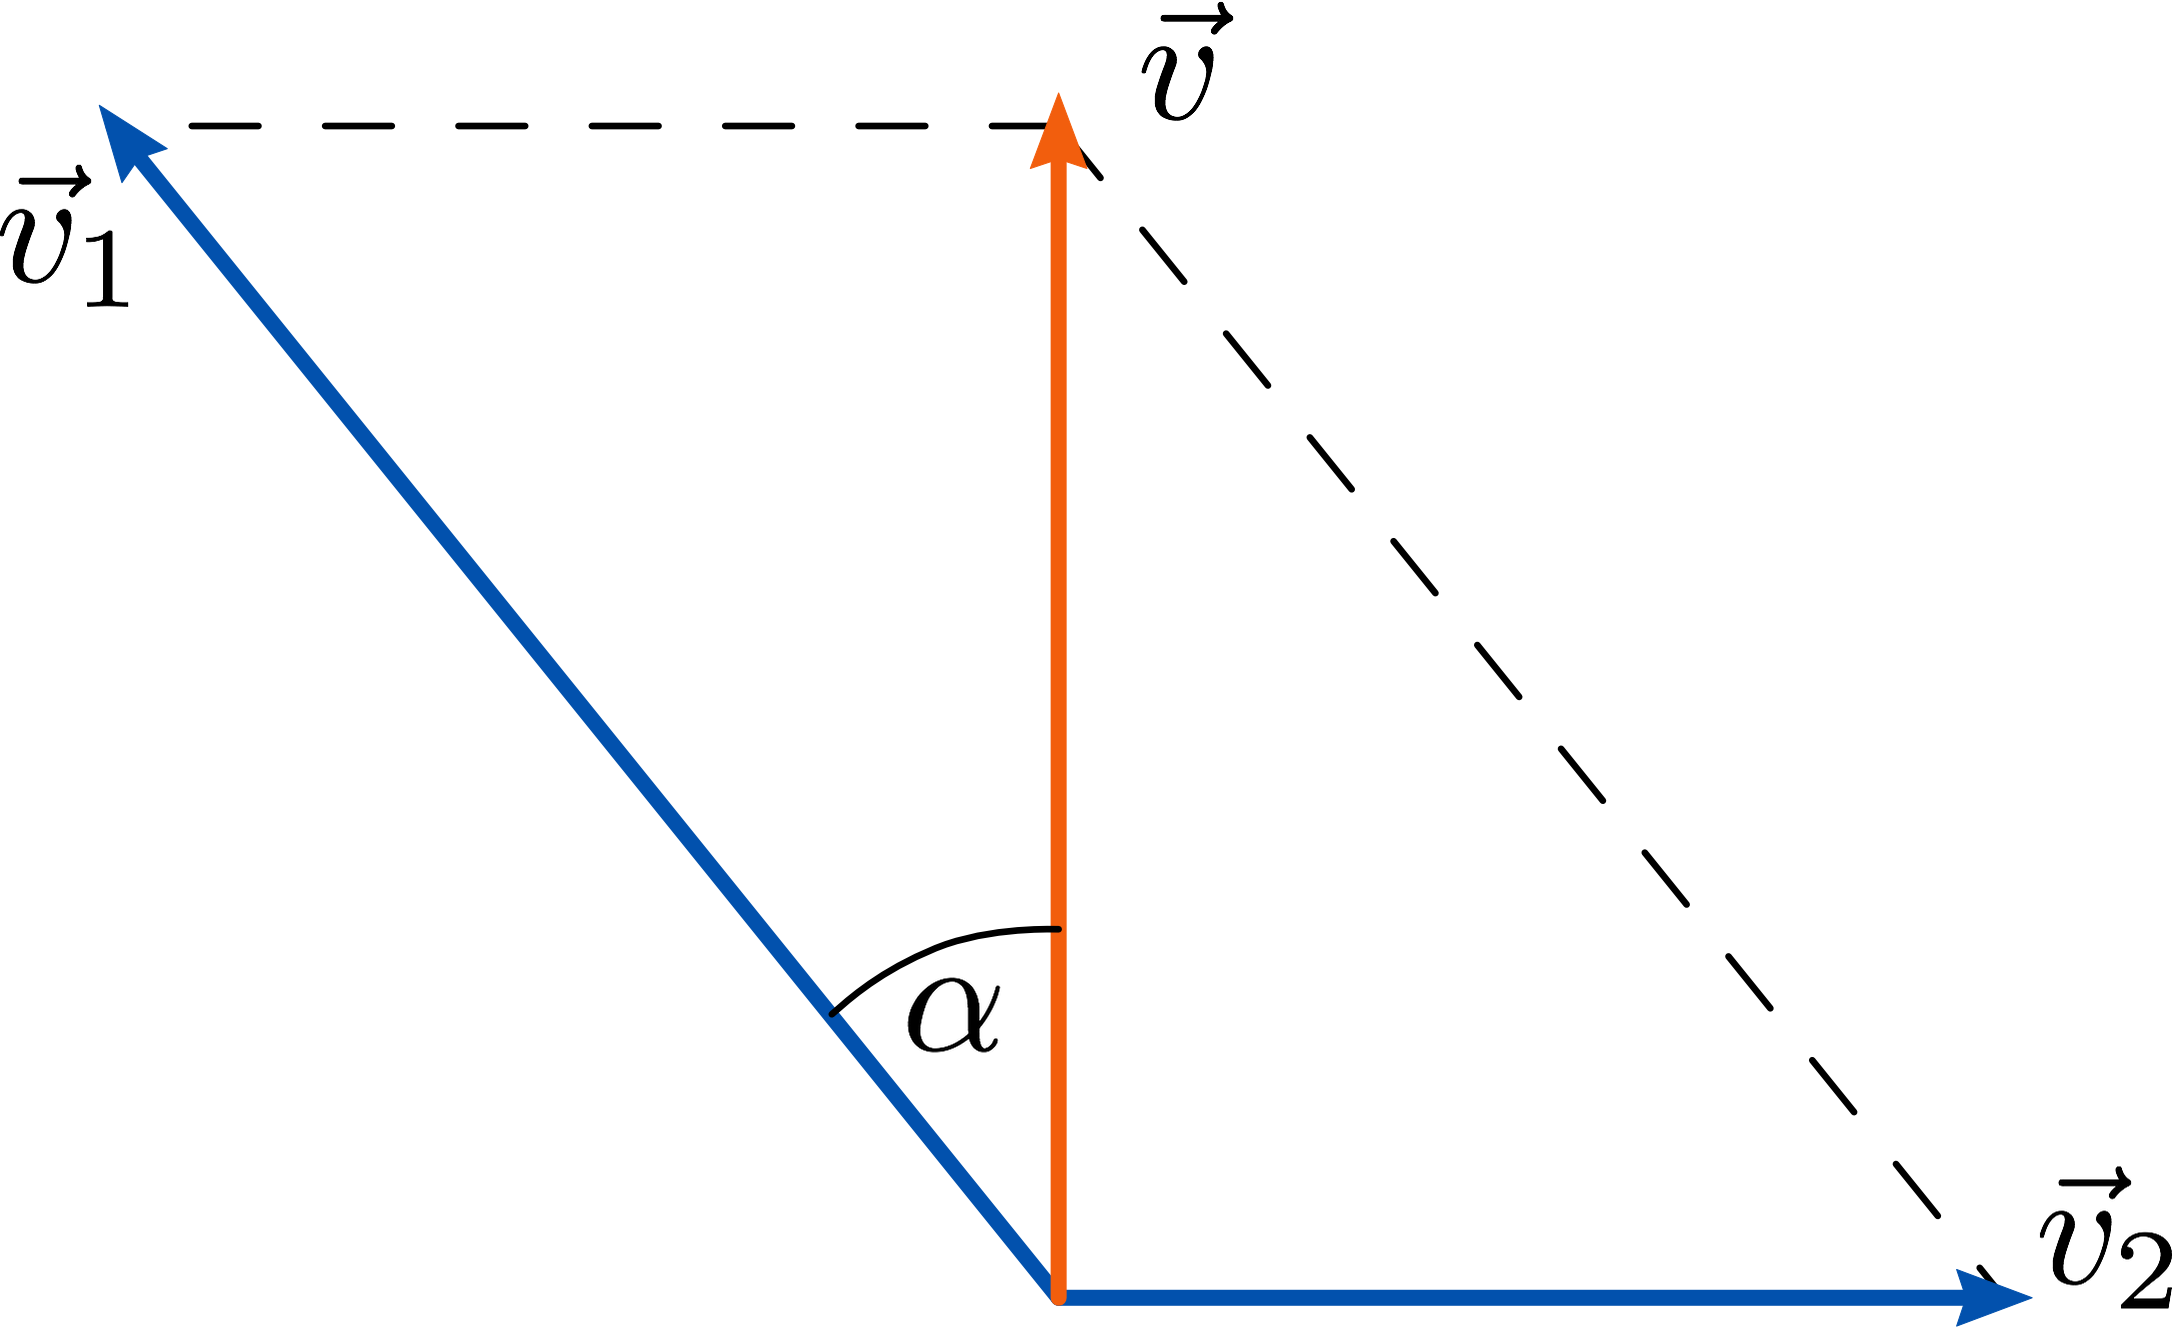
\includegraphics[width=0.45\textwidth]{dyn/exercises/vectoren_veerman}
\end{figure}
\newline
De hoek vinden we dan als volgt (zie figuur):
\begin{eqnarray*}
\sin{\alpha}&=&\frac{v_2}{v_1}\\
&\Downarrow&\\
\alpha&=&\bgsin\left(\frac{v_2}{v_1}\right)\\
&=&38,7^\circ
\end{eqnarray*}
De tijd nodig om de overzijde te bereiken vinden we door zijn snelheid loodrecht op de oever -- zijn resulterende snelheid $v$ -- te bekijken:
\begin{eqnarray*}
%v&=&v_1\cos{\alpha}\qquad\left(=v_1\cos\left(\bgsin\left(\frac{v_2}{v_1}\right)\right)=v_1\sqrt{1-\left(\frac{v_2}{v_1}\right)^2}=\sqrt{v_1^2-v_2^2}\right)\\
%&\Downarrow&\\
t&=&\frac{d}{v}=\frac{d}{\sqrt{v_1^2-v_2^2}}=96,1{\rm\,s}
\end{eqnarray*}
\end{oplossing}

\end{exercise}
